\documentclass[docid=2021]{comp_exam_round1}
\begin{document}
\setcounter{chapter}{2020}
\exam{Exam 2021}

\examgroup{}

Considering the following section of a grammar (parentheses and numbers on the right identify the productions), where ID is a token representing identifiers for variables and for names of functions, and TY is a token identifying data types (e.g., float, double, int, long):

\begin{itemize}[wide, noitemsep]
    \item \texttt{S → S Func | Func ~~~~~~~~~~~~~~~~~~~~~~~~~~~~~~~~~~~~~~~~~~~~(1, 2)}
    \item \texttt{Func → TY ID "(" Arg ")" ";" | TY ID "(" Arg ")" "\{" Body "\}" (3, 4)}
    \item \texttt{Arg → TY Arg1 | TY ID Arg1 | $\varepsilon$ ~~~~~~~~~~~~~~~~~~~~~~~~~~~~~~~(5, 6, 7)}
    \item \texttt{Arg1 → "," TY Arg1 | "," TY ID Arg1 | $\varepsilon$ ~~~~~~~~~~~~~~~~~~~~~~(8, 9, 10)}
    \item \texttt{Body → ...}
\end{itemize}

\question
Indicate the First and Follow sets for the grammar variables S, Func, Arg, and Arg1.

\ansseparator

\vspace{-2.0em}
\begin{alignat*}{5}
    & First(S   ) &&= \{ \texttt{TY}               \} && ~~~~~~~~~~ && Follow(S   ) &&= \{ \$, \texttt{TY} \} \\
    & First(Func) &&= \{ \texttt{TY}               \} && ~~~~~~~~~~ && Follow(Func) &&= \{ \$, \texttt{TY} \} \\
    & First(Arg ) &&= \{ \texttt{TY}, \varepsilon  \} && ~~~~~~~~~~ && Follow(Arg ) &&= \{ \texttt{")"}    \} \\
    & First(Arg1) &&= \{ \texttt{","}, \varepsilon \} && ~~~~~~~~~~ && Follow(Arg1) &&= \{ \texttt{")"}    \} \\
\end{alignat*}
\vspace{-3.0em}

\question
Considering only the variables S, Func, Arg, and Arg1, justify why the grammar is not LL(1) and show the LL(1) parsing table for those variables.

\ansseparator

\begin{center}
    \small
    \begin{tabular}{@{} c | p{25mm} | p{25mm} | p{25mm} | p{25mm} | p{25mm} @{}}
        \multirow{2}{*}{NT} & \multicolumn{5}{c}{T} \\ \cline{2-6}
               & \texttt{TY} & \texttt{","} & \texttt{")"} & \texttt{","} & \$ \\ \hline
        $S$    & 1, 2        &              &              &              &    \\ \hline
        $Func$ & 3, 4        &              &              &              &    \\ \hline
        $Arg$  & 5, 6        &              & 7            &              &    \\ \hline
        $Arg1$ &             & 8, 9         & 10           &              &   
    \end{tabular}
\end{center}

The grammar is not LL(1) because there is at least one cell which has more than one production, which means the LL(1) parser will have conflicts when parsing this language.

\question
Modify the variables, S, Func, Arg, and Arg1, in order that the grammar is LL(1) for those variables.

\ansseparator

\begin{itemize}[wide, noitemsep]
    \item \texttt{S → Func S'}
    \item \texttt{S' → Func S' | $\varepsilon$}
    \item \texttt{Func → TY ID "(" Arg ")" Func'}
    \item \texttt{Func' → ";" | "\{" Body "\}"}
    \item \texttt{Arg → TY Arg' | $\varepsilon$}
    \item \texttt{Arg' → Arg1 | ID Arg1 | $\varepsilon$}
    \item \texttt{Arg1 → "," TY Arg1' | $\varepsilon$}
    \item \texttt{Arg1' → Arg1 | ID Arg1 | $\varepsilon$}
\end{itemize}

\question
Modify the original grammar in order that the prototypes of the functions are distinguished from the non-prototypes, and that only the non-prototypes can have types with parameter names associated.

\ansseparator

\begin{itemize}[wide, noitemsep]
    \item \texttt{Func → Prot | TY ID "(" Arg ")" "\{" Body "\}"}
    \item \texttt{Prot → TY ID "(" ArgProt ")" ";"}
    \item \texttt{ArgProt → TY ArgProt1 | $\varepsilon$}
    \item \texttt{ArgProt1 → "," TY ArgProt1 | $\varepsilon$}
\end{itemize}

\examgroup{}

Consider the C code section presented in Code1, which includes the prototype of the “abs” function. This function is responsible to return the absolute value of the number passed as argument. Note that the integer literals are by default represented as “int” and the real literals are by default represented as “double” types.

\begin{lstlisting}[caption=Code1, language=c]
double abs(double);

float solve(float x) {
    float y = x;
    do {
        x = y;
        y = (2*x*x*x+5)/(3*x*x+1);
    } while(abs(x-y) >= 0.0001);
    return y;
}
\end{lstlisting}

\question
Show a symbol table for the function “solve” of Code1.

\ansseparator


\begin{center}
    \begin{tikzpicture}[every node/.style={align=center},level distance=7em]
        \Tree	[.{
                    Functions \\[0.5em]
                    \begin{tabular}{| c |}
                        \hline
                        ... \\ \hline
                        solve \\ \hline
                        ... \\ \hline
                    \end{tabular}
                }
                    {
                        Return \\
                        float
                        \vspace{0.5em}
                    }
                    {
                        Params \\[0.5em]
                        \begin{tabular}{| l |}
                            \hline
                            x (type: float) \\ \hline
                        \end{tabular}
                    }
                    {
                        Locals \\[0.5em]
                        \begin{tabular}{| l |}
                            \hline
                            y (type: float) \\ \hline
                        \end{tabular}
                    }
                ]
    \end{tikzpicture}
\end{center}

\question
Show a high-level intermediate representation (HLIR) for the function “solve” of Code1, based on the expression trees presented in lectures and output after semantic analysis. Note that the HLIR output must represent the adequate semantic analysis results.

\ansseparator


\vspace{-1em}
\begin{center}
    \ttfamily\small
    \begin{tikzpicture}
        \Tree	[.function
                    [.{stl y}
                        {ldp x}
                    ]
                    [.{do while}
                        [.{stp x}
                            {ldl y}
                        ]
                        [.{stl y}
                            [./
                                [.+
                                    [.*
                                        [.*
                                            [.*
                                                2
                                                {ldp x}
                                            ]
                                            {ldp x}
                                        ]
                                        {ldp x}
                                    ]
                                    5
                                ]
                                [.+
                                    [.*
                                        [.*
                                            3
                                            {ldp x}
                                        ]
                                        {ldp x}
                                    ]
                                    1
                                ]
                            ]
                        ]
                        [.$>=$
                            [.abs
                                [.-
                                    {ldp x}
                                    {ldl y}
                                ]
                            ]
                            0.0001
                        ]
                    ]
                ]
    \end{tikzpicture}
\end{center}

\examgroup{}

Comment the following sentence.

\question
In practice, the left recursion is not a problem for LL(k) as we can always define a lookahead value (k) sufficient large that make the implementation of the parser using left recursion feasible and efficient.

\ansseparator

False. Consider a language that can possibly have several functions, and that these functions are detected by the grammar using left recursion. Consider also that we are using a descendent syntactic analyser. Even if we choose an arbitrarily large value for $k$, we can always devise a new string with at least $k+1$ functions that the parser will struggle with.

Plus, left recursion may lead to infinite loops because the parser will apply the same production several times without ever checking if it matches the string to be matched.

\newpage

\examgroup{}

The Code2 example present a low-level three-address code intermediate representation (LLIR), where all the symbols (x, y, t0..t10) represent virtual 32-bit registers storing single-precision (32-bit) floating-point values and the constants are single-precision floating-point values. This LLIR is being used for compiling to a RISC CPU and each instruction in the LLIR has a direct CPU implementation.

\begin{lstlisting}[caption=Code2]
float solve( float x ) {
    float t0,t1,t2,t3,t4,t5;
    float t6,t7,t8,t9,t10;
    y = x;
L1:
    x = y;
    t0 = 2;
    t1 = t0*x;
    t2 = t1*x;
    t3 = t2*x;
    t4 = t3+5;
    t5 = 3;
    t6 = t5*x;
    t7 = t6*x;
    t8 = t7+1;
    y = t4/t8;
    t9 = x-y;
    t10 = absf(t9);
    if(t10 >= 0.0001) goto L1;
    return y;
}
\end{lstlisting}

\question
Draw the control-flow graph (CFG) for Code2 (identify the instruction in each node by using the respective line number).

\ansseparator

\begin{center}
    \small
    \begin{tikzpicture}[->,>=stealth',node distance=3.5em, initial text=$ $,]
        \node[chamfered rectangle, chamfered rectangle xsep=1cm, draw] (1)  {Start (1)};
        \node[draw, right =2em of 1] (2)  {2};
        \node[draw, right of= 2] (3)  {3};
        \node[draw, right of= 3] (4)  {4};
        \node[draw, right of= 4] (6)  {6};
        \node[draw, right of= 6] (7)  {7};
        \node[draw, right of= 7] (8)  {8};
        \node[draw, right of= 8] (9)  {9};
        \node[draw, right of= 9] (10) {10};
        \node[draw, right of=10] (11) {11};
        \node[draw, right of=11] (12) {12};
        \node[draw, below of=12] (13) {13};
        \node[draw, left  of=13] (14) {14};
        \node[draw, left  of=14] (16) {16};
        \node[draw, left  of=16] (17) {17};
        \node[draw, left  of=17] (18) {18};
        \node[draw, left  of=18] (19) {19};
        \node[draw, below of=19] (20) {20};
     
        \draw	   
            (1)    edge    (2)
            (2)    edge    (3)
            (3)    edge    (4)
            (4)    edge    (6)
            (6)    edge    (7)
            (7)    edge    (8)
            (8)    edge    (9)
            (9)    edge    (10)
            (10)   edge    (11)
            (11)   edge    (12)
            (12)   edge    (13)
            (13)   edge    (14)
            (14)   edge    (16)
            (16)   edge    (17)
            (17)    edge    (18)
            (18)    edge    (19)
            (19)    edge[right] node{yes} (6)
            (19)    edge[right] node{no} (20)
        ;

    \end{tikzpicture}
\end{center}

\newpage

\question
By inspecting Code2, draw the interference graph (IG) considering the virtual registers.

\ansseparator

\noindent
\begin{minipage}{\textwidth}
\begin{center}
    \setlength{\tabcolsep}{0.48em}
    \begin{tabular}{l | c c c c c c c c c c c c c}
                                                & x       & y       & t0      & t1      & t2      & t3      & t4      & t5      & t6      & t7      & t8      & t9      & t10     \\ \hline
        \texttt{ 2. float t0,t1,t2,t3,t4,t5;}   & $\vert$ &         &         &         &         &         &         &         &         &         &         &         &         \\ \hline
        \texttt{ 3. float t6,t7,t8,t9,t10;}     & $\vert$ &         &         &         &         &         &         &         &         &         &         &         &         \\ \hline
        \texttt{ 4. y = x;}                     & $\bot$  & $\top$  &         &         &         &         &         &         &         &         &         &         &         \\ \hline
        \texttt{ 5. L1:}                        &         & $\vert$ &         &         &         &         &         &         &         &         &         &         &         \\ \hline
        \texttt{ 6. x = y;}                     & $\top$  & $\bot$  &         &         &         &         &         &         &         &         &         &         &         \\ \hline
        \texttt{ 7. t0 = 2;}                    & $\vert$ &         & $\top$  &         &         &         &         &         &         &         &         &         &         \\ \hline
        \texttt{ 8. t1 = t0*x;}                 & $\vert$ &         & $\bot$  & $\top$  &         &         &         &         &         &         &         &         &         \\ \hline
        \texttt{ 9. t2 = t1*x;}                 & $\vert$ &         &         & $\bot$  & $\top$  &         &         &         &         &         &         &         &         \\ \hline
        \texttt{10. t3 = t2*x;}                 & $\vert$ &         &         &         & $\bot$  & $\top$  &         &         &         &         &         &         &         \\ \hline
        \texttt{11. t4 = t3+5;}                 & $\vert$ &         &         &         &         & $\bot$  & $\top$  &         &         &         &         &         &         \\ \hline
        \texttt{12. t5 = 3;}                    & $\vert$ &         &         &         &         &         & $\vert$ & $\top$  &         &         &         &         &         \\ \hline
        \texttt{13. t6 = t5*x;}                 & $\vert$ &         &         &         &         &         & $\vert$ & $\bot$  & $\top$  &         &         &         &         \\ \hline
        \texttt{14. t7 = t6*x;}                 & $\vert$ &         &         &         &         &         & $\vert$ &         & $\bot$  & $\top$  &         &         &         \\ \hline
        \texttt{15. t8 = t7+1;}                 & $\vert$ &         &         &         &         &         & $\vert$ &         &         & $\bot$  & $\top$  &         &         \\ \hline
        \texttt{16. y = t4/t8;}                 & $\vert$ & $\top$  &         &         &         &         & $\bot$  &         &         &         & $\bot$  &         &         \\ \hline
        \texttt{17. t9 = x-y;}                  & $\bot$  & $\vert$ &         &         &         &         &         &         &         &         &         & $\top$  &         \\ \hline
        \texttt{18. t10 = absf(t9);}            &         & $\vert$ &         &         &         &         &         &         &         &         &         & $\bot$  & $\top$  \\ \hline
        \texttt{19. if(t10 >= 0.0001) goto L1;} &         & $\vert$ &         &         &         &         &         &         &         &         &         &         & $\bot$  \\ \hline
        \texttt{20. return y;}                  &         & $\bot$  &         &         &         &         &         &         &         &         &         &         &         \\
    \end{tabular}
\end{center}
\end{minipage}

\begin{center}
    \footnotesize
    \begin{tikzpicture}[-,>=stealth',node distance=4.5em,initial text=$ $,]
        \node[state                   ] (x)   {x};
        \node[state,       above of=x ] (t1)  {t1};
        \node[state,       left  of=t1] (t0)  {t0};
        \node[state,       right of=t1] (t2)  {t2};
        \node[state,       right of=t2] (t3)  {t3};
        \node[state,       left  of=t0] (y)   {y};
        \node[state, below left  of=x] (t6)  {t6};
        \node[state,       left of=t6] (t5)  {t5};
        \node[state, below right of=x ] (t7)  {t7};
        \node[state,       right of=t7] (t8)  {t8};
        \node[state, above left  of=y ] (t9)  {t9};
        \node[state, above right of=y ] (t10) {t10};
        \node[state, below right of=t6] (t4)  {t4};
        
        \draw   
                (x)	    edge (y)
                (x)	    edge (t0)
                (x)	    edge (t1)
                (x)	    edge (t2)
                (x)	    edge (t3)
                (x)	    edge (t4)
                (x)	    edge (t5)
                (x)	    edge (t6)
                (x)	    edge (t7)
                (x)	    edge (t8)
                (y)     edge (t9)
                (y)     edge (t10)
                (t4)    edge (t5)
                (t4)    edge (t6)
                (t4)    edge (t7)
                (t4)    edge (t8)
                ;

    \end{tikzpicture}
\end{center}

\newpage

\question
Show the results of applying a first iteration of register allocation (with the graph-coloring based algorithm presented in lectures) and considering that virtual registers “x” and “y” must be allocated to R2 and R3, respectively, and the other register available is R4. Show the LLIR after this first iteration of register allocation and to be used in the next iteration. If used, describe coalescing, freeze, and register spilling, and how did you select the register(s) to spill.

\ansseparator

\noindent
\begin{minipage}{0.20\textwidth}
\begin{center}
    \begin{tabular}{| c |}
        \textbf{Stack top} \\ \cline{1-1}
        t4 \\
        x \\
        t8 \\
        t7 \\
        t6 \\
        t5 \\
        y \\
        t10 \\
        t9 \\
        t3 \\
        t2 \\
        t1 \\
        t0 \\ \cline{1-1}
        \textbf{Stack bottom}
    \end{tabular}
\end{center}
\end{minipage}
\begin{minipage}{0.27\textwidth}
    R2 = \{x, t9, t10\} \\
    R3 = \{y, t0, t1, t2, t3, t4\} \\
    R4 = \{t5, t6, t7, t8\}
\end{minipage}
\begin{minipage}{0.51\textwidth}
\begin{center}
    \footnotesize
    \begin{tikzpicture}[-,>=stealth',node distance=4.5em,initial text=$ $,]
        \node[state                   , fill=red!30  ] (x)   {x};
        \node[state,       above of=x , fill=green!30] (t1)  {t1};
        \node[state,       left  of=t1, fill=green!30] (t0)  {t0};
        \node[state,       right of=t1, fill=green!30] (t2)  {t2};
        \node[state,       right of=t2, fill=green!30] (t3)  {t3};
        \node[state,       left  of=t0, fill=green!30] (y)   {y};
        \node[state, below left  of=x , fill=blue!30 ] (t6)  {t6};
        \node[state,       left of=t6 , fill=blue!30 ] (t5)  {t5};
        \node[state, below right of=x , fill=blue!30 ] (t7)  {t7};
        \node[state,       right of=t7, fill=blue!30 ] (t8)  {t8};
        \node[state, above left  of=y , fill=red!30  ] (t9)  {t9};
        \node[state, above right of=y , fill=red!30  ] (t10) {t10};
        \node[state, below right of=t6, fill=green!30] (t4)  {t4};
        
        \draw   
                (x)	    edge (y)
                (x)	    edge (t0)
                (x)	    edge (t1)
                (x)	    edge (t2)
                (x)	    edge (t3)
                (x)	    edge (t4)
                (x)	    edge (t5)
                (x)	    edge (t6)
                (x)	    edge (t7)
                (x)	    edge (t8)
                (y)     edge (t9)
                (y)     edge (t10)
                (t4)    edge (t5)
                (t4)    edge (t6)
                (t4)    edge (t7)
                (t4)    edge (t8)
                ;

    \end{tikzpicture}
\end{center}
\end{minipage}

\question
Draw the data-dependence graph (DDG) for the lines from 7 to 17 of Code2 (identify each node by the respective line number). Consider that each assignment to a constant can be implemented by an arithmetic instruction of the target machine.

\ansseparator

\noindent
The dependency graph is:

\begin{center}
    \footnotesize
    \begin{tikzpicture}[->,>=stealth',node distance=3.5em,initial text=$ $,]
        \node[state                     ] (17)  {17};
        \node[state, above       of=17  ] (16)  {16};
        \node[state, above right of=16  ] (15)  {15};
        \node[state, above       of=15  ] (14)  {14};
        \node[state, above       of=14  ] (13)  {13};
        \node[state, above       of=13  ] (12)  {12};
        \node[state, above left  of=16  ] (11)  {11};
        \node[state, above       of=11  ] (10)  {10};
        \node[state, above       of=10  ] (9)   {9};
        \node[state, above       of=9   ] (8)   {8};
        \node[state, above       of=8   ] (7)   {7};
        
        \draw	   
                (16)    edge    (17)
                (15)    edge    (16)
                (14)    edge    (15)
                (13)    edge    (14)
                (12)    edge    (13)
                (11)    edge    (16)
                (10)    edge    (11)
                (9)     edge    (10)
                (8)     edge    (9)
                (7)     edge    (8)
                ;

    \end{tikzpicture}
\end{center}

\question
Considering that in the target machine all instructions execute in 1 clock cycle, and the machine has a single unit for all instructions, indicate how many clock cycles are needed for executing the instructions in the DDG.

\ansseparator

\noindent
It takes 11 cycles to execute the instructions in the DDG, because there is no parallelism, all instructions execute in 1 cycle and there are 11 instructions.

\question
Considering that in the target machine all instructions execute in 1 clock cycle, and the machine has two units able to execute any arithmetic/logic instruction, present the scheduling of instructions resultant of applying the list-scheduling algorithm to the DDG, and the number of clock cycles needed to execute the instructions in the DDG. Show the values used for the criterion to select between the instructions in the DDG.

\ansseparator

\noindent
The dependency graph (with height in parenthesis) is:

\begin{center}
    \small
    \begin{tikzpicture}[->,>=stealth',node distance=4.0em,initial text=$ $,]
        \node[state                     ] (17)  {17}; \node[right=0em of 17 ] (17d) {(1)};
        \node[state, above       of=17  ] (16)  {16}; \node[right=0em of 16 ] (16d) {(2)};
        \node[state, above right of=16  ] (15)  {15}; \node[right=0em of 15 ] (15d) {(3)};
        \node[state, above       of=15  ] (14)  {14}; \node[right=0em of 14 ] (14d) {(4)};
        \node[state, above       of=14  ] (13)  {13}; \node[right=0em of 13 ] (13d) {(5)};
        \node[state, above       of=13  ] (12)  {12}; \node[right=0em of 12 ] (12d) {(6)};
        \node[state, above left  of=16  ] (11)  {11}; \node[right=0em of 11 ] (11d) {(3)};
        \node[state, above       of=11  ] (10)  {10}; \node[right=0em of 10 ] (10d) {(4)};
        \node[state, above       of=10  ] (9)   {9 }; \node[right=0em of 9  ] (9d)  {(5)};
        \node[state, above       of=9   ] (8)   {8 }; \node[right=0em of 8  ] (8d)  {(6)};
        \node[state, above       of=8   ] (7)   {7 }; \node[right=0em of 7  ] (7d)  {(7)};
        
        \draw	   
                (16)    edge    (17)
                (15)    edge    (16)
                (14)    edge    (15)
                (13)    edge    (14)
                (12)    edge    (13)
                (11)    edge    (16)
                (10)    edge    (11)
                (9)     edge    (10)
                (8)     edge    (9)
                (7)     edge    (8)
                ;

    \end{tikzpicture}
\end{center}

To select among ready instructions, we first choose those that have greatest height (distance from the last node); we break ties by selecting the instruction that appears first in the code.

\begin{center}
    \begin{tabular}{c | c c}
        \textbf{Cycle}  & \textbf{FU1} & \textbf{FU2} \\ \hline
        1               & 7            & 12           \\
        2               & 8            & 13           \\
        3               & 9            & 14           \\
        4               & 10           & 15           \\
        5               & 11           &              \\
        6               & 16           &              \\
        7               & 17           &              \\
    \end{tabular}
\end{center}

\examgroup{}

\question
Consider that Code2 is represented as a CFG consisting of nodes that represent each instruction as an expression tree. Describe your suggestion to do instruction selection using Maximal Munch and considering that besides the direct implementation of three-address code instructions by the target machine, the machine also includes native support for single-precision floating-point instructions: dst = c*src1*src2; and dst = src1*src2+c; (where dst, src1, and src2 are 32-bit registers and c is a single-precision floating-point constant). Show the region of the CFG where instruction selection may select these instructions and how they are identified.

\ansseparator

\noindent
First of all, I suggest generating the AST tiles for these two new operations. We assume the AST will be built by considering that all operations are left-associative, to reduce the number of possible tiles.

\begin{center}
    \begin{tabular}{c | c}
        \textbf{Operation 1: } \texttt{dst = c*src1*src2} & \textbf{Operation 2: } \texttt{dst = src1*src2+c} \\ \hline
        \begin{minipage}{0.16\textwidth}
            \begin{center}
                \ttfamily\small
                \begin{tikzpicture}
                    \Tree	[.*
                                [.*
                                    c
                                    src1
                                ]
                                src2
                            ]
                \end{tikzpicture}
            \end{center}
        \end{minipage}%
        \begin{minipage}{0.16\textwidth}
            \begin{center}
                \ttfamily\small
                \begin{tikzpicture}
                    \Tree	[.*
                                [.*
                                    src1
                                    c
                                ]
                                src2
                            ]
                \end{tikzpicture}
            \end{center}
        \end{minipage}%
        \begin{minipage}{0.16\textwidth}
            \begin{center}
                \ttfamily\small
                \begin{tikzpicture}
                    \Tree	[.*
                                [.*
                                    src1
                                    src2
                                ]
                                c
                            ]
                \end{tikzpicture}
            \end{center}
        \end{minipage}%
        &
        \begin{minipage}{0.16\textwidth}
            \begin{center}
                \ttfamily\small
                \begin{tikzpicture}
                    \Tree	[.+
                                [.*
                                    src1
                                    src2
                                ]
                                c
                            ]
                \end{tikzpicture}
            \end{center}
        \end{minipage}%
        \begin{minipage}{0.16\textwidth}
            \begin{center}
                \ttfamily\small
                \begin{tikzpicture}
                    \Tree	[.+
                                c
                                [.*
                                    src1
                                    src2
                                ]
                            ]
                \end{tikzpicture}
            \end{center}
        \end{minipage}%
    \end{tabular}
\end{center}

As can be seen, each operation has more than one possible tiling. This will allow us to detect all situations where these two operations might be applied.

\begin{center}
    \begin{tabular}{@{} p{77mm} p{77mm} @{}}
        The AST of the main cycle of Code2 is: & The new operations can be applied in the following situations (operation 1 in full, operation 2 dashed): \\
        \begin{minipage}{\linewidth}
            \centering
            \ttfamily\small
            \begin{tikzpicture}
                \Tree	[.absf
                            [.-
                                x
                                [./
                                    [.+
                                        [.*
                                            [.*
                                                [.*
                                                    2
                                                    x
                                                ]
                                                x
                                            ]
                                            x
                                        ]
                                        5
                                    ]
                                    [.+
                                        [.*
                                            [.*
                                                3
                                                x
                                            ]
                                            x
                                        ]
                                        1
                                    ]
                                ]
                            ]
                        ];
            \end{tikzpicture}
        \end{minipage}%
        &
        \begin{minipage}{\linewidth}
            \centering
            \ttfamily\small
            \begin{tikzpicture}
                \Tree	[.absf
                            [.-
                                x
                                [./
                                    [.+
                                        [.*
                                            [.*
                                                [.*
                                                    2
                                                    x
                                                ]
                                                x
                                            ]
                                            x
                                        ]
                                        5
                                    ]
                                    [.+
                                        [.*
                                            [.*
                                                3
                                                x
                                            ]
                                            x
                                        ]
                                        1
                                    ]
                                ]
                            ]
                        ];

                \draw [rounded corners=4mm] (-0.4,-4.5) -- ++(-1.4, -3.1) -- ++(+1.6,0) -- ++(0.65, 1.4) -- cycle;
                \draw [rounded corners=4mm] (+2.1,-3.5) -- ++(-1.4, -3.1) -- ++(+1.6,0) -- ++(0.65, 1.4) -- cycle;

                \draw [rounded corners=4mm, dashed] (+0.5,-2.4) -- ++(-0.9, -1.7) -- ++(+0.9,-1.7) -- ++(0.9, 1.7) -- cycle;
                \draw [rounded corners=4mm, dashed] (+2.55,-2.4) -- ++(-0.9, -1.7) -- ++(+0.9,-1.7) -- ++(0.9, 1.7) -- cycle;
            \end{tikzpicture}
        \end{minipage}%
    \end{tabular}
\end{center}

We know the largest tiles are those mapping to these two new operations, because all other operations are three-address codes, and these two operations are four-address codes.

Now we only have to apply Maximal Munch: starting at the root, for the current node try to fit the largest tile possible. When running the Maximal Munch algorithm, the left side of \texttt{/} is covered with one operation 1 and one operation 2; the right side is only covered with one operation 2 and the rest is done with three-address codes, because the operation 2 on the right branch of \texttt{/} partially covers the operation 1, and because the operation 2 root is closer to the root, operation 2 will be assigned first and the operation 1 will no longer fit.

\end{document}
